\documentclass{article} % Document class
\usepackage{amsmath, bm, amssymb,amsthm,enumitem}
\usepackage{tikz}
\usetikzlibrary{arrows}
\usepackage{babel}[english]
\usepackage{pgfplots}
\usepackage{titlesec}
\usepackage{lipsum}
\pgfplotsset{compat=1.18}
\usepackage{siunitx}                    % new
\usepackage{xparse}                     % new
\title{My bs notes}
\author{Makus}
\date{\today}

\usepackage{booktabs, multirow, threeparttable}   % new
\newtheorem{exmp}{Example}[paragraph]
\newtheorem{problem}{Problem}
\setcounter{secnumdepth}{4}
\theoremstyle{theorem}
\newtheorem{theorem}{Theorem}[paragraph]
\titleformat{\paragraph}
{\normalfont\normalsize\bfseries}{\theparagraph}{1em}{}
\titlespacing*{\paragraph}
{0pt}{3.25ex plus 1ex minus .2ex}{1.5ex plus .2ex}
\renewcommand{\qedsymbol}{$QED$}
\newtheorem{exmat}{Example}[subsection]
\theoremstyle{definition}
\newtheorem{definition}{Definition}

\begin{document} % Begin document content
\maketitle

% \grouping{<something>} acts similar to a ToC entry for \chapter*{<something>}
%\pgfplotsset{ standard/.style={ axis line style = thick, trig format=rad, enlargelimits, axis x line=middle, axis y line=middle, enlarge x limits=0.15, enlarge y limits=0.15, every axis x label/.style={at{(current axis.right of origin)},anchor=north west}, every axis y label/.style={at={(current axis.above of origin)},anchor=south east} } }
\setcounter{tocdepth}{5}
\tableofcontents
\pagebreak
\section{Introduction}
    \begin{center}
        just random ass notes, separted by sections.
    \end{center}
    \subsection{forenotes}
    For the entire part of Computer Science, Chapter 3, the variable naming standard will be as follows:
    \begin{center}
        i is input\\ o is output
    \end{center}
    unless stated otherwise.
    \\Another note is that the $QED$, meaning \textit{quod erat demonstratum} in Latin, means ''it is demonstrated'' and marks the end of proofs.
\pagebreak
\section{math}% ! math
    \subsection{general}
        \subsubsection{bases}
        given  \begin{center}
            $n$ = base of number representation\\
            $x$ = number that is represented in base $n$,
        \end{center}
        Then $\dfrac{x}{n}$ shiftes everything in $x$ towards the left by one and $x\cdot n$ shiftes everything to the right.
        \subsubsection{logrithmic base 2}
        when taking $\log_2(1+x)$ where $0<x \leq1$, the output is approx. $x$.\\
        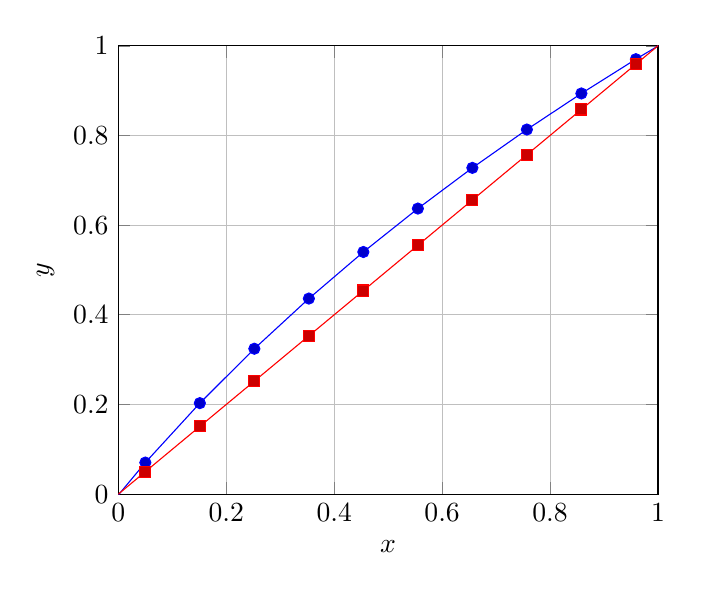
\begin{tikzpicture}
            \begin{axis}[
                xlabel={$x$},
                ylabel={$y$},
                samples=100,
                grid=major,
                xmin=0,xmax=1,
                ymin=0,ymax=1]
                \addplot{log10(x+1)/log10(2)};
                \addplot{x};
            \end{axis}
        \end{tikzpicture}
        \\but by adding $\mu$ to this, we can lower the amount of error to the average.
        to find $\mu$, we can do a mean value theorem stated in calculus portion to find $\mu$, which can be gotten from
        \begin{center}
            if$f(x)=\log_2(x+1)$, then $$f'(x)=\dfrac{1}{(x+1)\ln(2)}$$since the average rate of change is $$\dfrac{f(1)-f(0)}{1-0}=1$$
            then to get $\mu$, the steps are $$f'(c)=\dfrac{1}{(c+1)\ln(2)}=1$$ $$1=(c+1)\ln(2)$$ $$c=\dfrac{1}{\ln(2)}-1$$
            solving for c gives us the point on $f(x)$ where $f'(c)=1$
            \\given $c=\dfrac{1}{\ln(2)}-1$, then we can graph the tangent line with the point slope form.\\ $y-f(c)=f'(c)(x-c)$, or
            $$y=f(c)+f'(c)(x-c)$$ or $$y=f(c)-c+x$$ since $f'(c)=1$. since $f(c)-c$ is constant, it would be a straight line, modeled by the green line in the following
            the green line shows the tangent line with least error throughout. In order to find the overall average error, we can divide the sum of y intercepts by two in order to get the value of $\mu$, modeled by the blue line.
            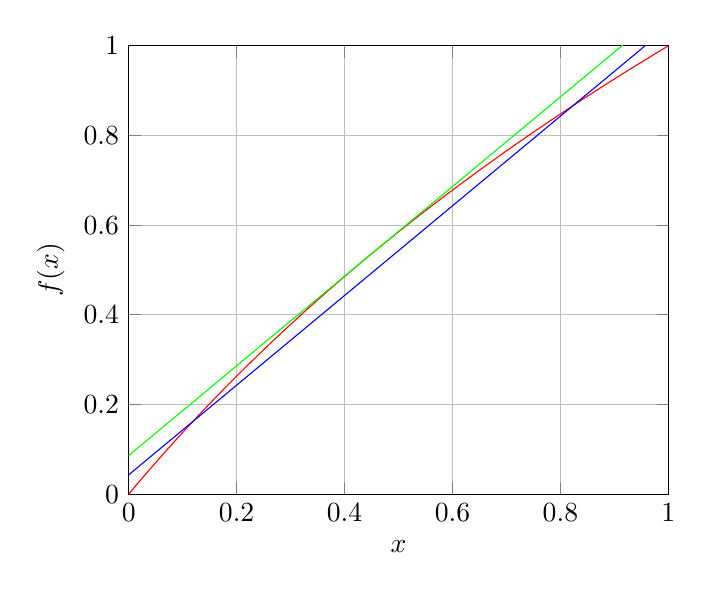
\begin{tikzpicture}
                \begin{axis}[xlabel={$x$},ylabel={$f(x)$},xmin=0, xmax=1,ymin=0,ymax=1,samples=1000,grid=major]
                    \addplot[color=red]{log10(x+1)/log10(2)};
                    \addplot[color=green]{x-(1/ln(2)-1)+log10(1/ln(2))/log10(2)} node[right]{$x+c$};
                    \addplot[color=blue]{x-((1/ln(2)-1)-log10(1/ln(2))/log10(2))/2};
                \end{axis}
            \end{tikzpicture}
            red is $\log_2(x+1)$\\
            green is $x+c-f(c)$, where $f(c)=\log_2(x+1)$\\
            blue is $x+\mu$, where $\mu=\dfrac{f(c)-c}{2}$
        \end{center}
    \subsection{Vector/Matrix math} % (fold)
    \label{sub:vecMat}
        \subsubsection{basics}
        %note: vector math
            Vectors have different definitions depending on the discipline, Math and Computer Science, but this section will ignore the Computer Science aspect.
            This is how normal matrices are denoted:
            \[\begin{bmatrix}
                e_1 & e_2 & e_3 & \\
                1 & 2 & 3 & d_1\\
                a & b & c & d_2
            \end{bmatrix}=M\]
            Each element can be denoted through $m_{d,e}$, where $e$ is the column and $d$ is the row .
            \begin{exmat}
                \[
                    m_{1,2}=2, m_{2,3}=c
                \]
            \end{exmat}
            matrix can be used to represent data.
        \subsubsection{operations} % (fold)
        \label{ssub:operations}
            \paragraph{scalar multiplication}
                What this means is that if $c_0\cdot M$, then that means 
                \[ c_0\cdot M = \begin{bmatrix}
                    c_0\cdot 1 &c_0\cdot 1 &c_0\cdot 1 \\
                    c_0\cdot a & c_0\cdot b &c_0\cdot c
                \end{bmatrix} \]
        
        % subsection vecMat (end)
    \pagebreak
    \subsection{calculus}
    this section will follow the order in which Calculus BC is taught, with first half from start of school to optimization problems, and second half being from integration to everything else.
        \subsubsection{First Half}
        This will mostly be derivatives and AB stuff.
            \paragraph{Mean Value Theorem} % (fold)
            \label{ssub:Mean Value Theorem}
                Mean Value Theorem, or MVT, states that if f(x) is continuous and differentiable within the range $a\le x \le b$, then there exists a point $c$ where $f'(c) = \dfrac{f(b)-f(a)}{b-a}$
        \subsubsection{Second Half}
            \paragraph{Unit 5}
                \subparagraph{Integration}
                    it is the inverse of differentiation, much like addition and subtraction. This process is denoted with the equation below.
                    $$\int f'(x)dx = f(x)$$
                    This shows the process of integration. A basic integration technique is Riemann sums.
                \subparagraph{Riemann Sums}
                    This is where we draw rectangles from the axis from which the function is in terms of up to a point of a function. Each subinterval's width can be given or can be calculated by a simple division. There are different types of Riemann sums.
                    It is not necessarily a rectangle, but it can also be a trapezoid, which is called the trapezoid Riemann Sum.
                    Some examples of Riemann Sums are:
                    \begin{itemize}
                        \item right corner: the height of the rectangle is equal to the value of the function at the right bound/limit, and can be modeled by the function $$\int_a^\beta f(x)\approx \sum_{k=1}^{n}f(a+k \cdot \Delta x)\cdot\Delta x$$
                        \item left corner: the height of the rectangle is equal to the value of the function at the left bound/limit, and can be modeled by the function $$\int_a^\beta f(x) \approx \sum_{k=1}^{n}f(a+(k-1)\cdot \Delta x)\cdot\Delta x$$
                        \item midpoint: the height of the rectangle is equal to the value of the function in the middle of the bound/limit, and can be modeled by the function $$\int_a^\beta f(x)\approx \sum_{k=1}^{n}f(a+(\Delta x\cdot(k-1))+(\frac{\Delta x}{2}))$$
                    \item trapezoid: instead of rectangles, trapezoids are used. This can be modeled by the function $$\int_a^\beta f(x)\approx \sum_{k=1}^{n}(f(a+(k-1)\cdot\Delta x)+f(a+k\cdot\Delta x))\frac{\Delta x}{2}$$
                    \end{itemize}
                    where the variables are designed as
                    \begin{center}
                        $\Delta x$ is the width of the subinterval of each subinterval\\
                        $a$ is the lower limit/bound of the integral\\
                        $\beta$ is the upper limit/bound of the integral\\
                        $n$ is the number of subintervals specified\\
                    \end{center}
                    Note: $n$ can be calculated if $a$ and $\beta$
                    If something isn't integratable, then U-substitution can be used.
                    the Riemann sums function is defined by the equation:
                    \begin{equation}
                        \int^b_a f(x)dx = \lim_{n \to \infty} \sum_{k=1}^{n}f(c_k)\Delta x_k
                    \end{equation}
                    where $\Delta x_k$ is $\frac{b-a}{n}$, and $c_k$ is $a+\Delta x_k \cdot k$
                \subparagraph{U substitution}
                    A variable can be used to replace a portion of a function. How this will work is:
                    \begin{enumerate}
                        \item Substitute a part of the function as u.
                        \item Where $u = f(x)$, the derivative would be $\dfrac{du}{dx} = f'(x)$, or $du = f'(x)dx$
                        \item Isolate dx an whatever way needed, then replace it back into the original function, so that the integral will be in terms of u (meaning it would be $\int du$)
                        \item After integrating, replace $u$ with $f(x)$
                    \end{enumerate}
                    Following these steps would look something like:
                    \begin{align*}
                        \int \dfrac{x}{\sqrt{1-4x^2}}dx \hspace{30px}
                        u &= 1-4x^2\\
                        \dfrac{du}{dx} &= 8x\\
                        du&=8xdx \\
                        \int \dfrac{1}{\sqrt{u}}du \hspace{80px}\\
                        \int u^{-1/2}du \hspace{70px}\\
                        \int u^{-\frac{1}{2}}du = \dfrac{u^{\frac{1}{2}}}{\frac{1}{2}}+c\hspace{30px}\\
                        2(1-4x^2)^{\frac{1}{2}}+c\hspace*{50px}
                    \end{align*}
                    If there are still $x$ values left after U-sub, then algabraic substitution can be used. This is where $u$ is expressed in terms of $x$.
                \subparagraph{Definite Integrals}
                    definite integrals output the area beneath the curve of the function, with the bounds of $a$ and $\beta$, where $a<\beta$. Notation denoted below:
                    $$\int_{a}^{\beta}f'(x) dx = [f(x)]^{x=a}_{x=\beta}$$ 
                    if $a$ and $\beta$ are switched, then:
                    $$\int_{\beta}^{a}f'(x) dx = -[f(x)]^{x=a}_{x=\beta}$$
                    some more properties include:
                    \begin{enumerate}
                        \item $\int ^{a}_{a}f(x)dx = 0$
                        \item $\int _{a}^{\beta}cf(x)dx =c\int _{a}^{\beta}f(x)dx$(including negative numbers)
                        \item $\int _{a}^{\beta}(f(x)\pm g(x))dx = \int _{a}^{\beta}f(x)dx\pm \int _{a}^{\beta} g(x)dx$
                        \item $\int _{a}^{\beta}(f(x)dx)+\int ^{\gamma}_{a}(f(x)dx)=\int ^{\gamma}_{a}(f(x)dx)$
                        \item $\int ^{a}_{-a}f(x)dx=2\int ^{a}_{0}f(x)dx$ assuming f(x) is even
                        \item $\int ^{a}_{-a}f(x)dx=0$ assuming f(x) is odd
                    \end{enumerate}
                \subparagraph{Fundamental Theorem of Calculus part 1}
                \label{subp:FTCpt1}
                    If $f$ is continuous on $[a,b]$, then the following would be true:
                    \begin{equation}
                        \int^\beta_a f'(x)dx = [f(x)]^{x=\beta}_{x=a}=f(b)-f(a)
                    \end{equation}
                    Given this, it is possible to find either one of the three terms given two. 
                    \\\textbf{Keep In Mind}, when using U substitution and difinite integrals, the bounds need to change accordingly.
                    \begin{equation}
                        \int^\beta_a f(u(x))u'(x)dx = \int^{u(\beta)}_{u(a)}f(u)du
                    \end{equation}
                \subparagraph{Average Value}
                The function defines the formula to find the average value of a function. Given that we have to find the average value of $f$ on the interval $[a,b]$his is defined by: 
                    \begin{equation}
                        f_{avg}=\frac{1}{b-a}\int_{a}^{b}f(x)dx
                        \label{eq:avgValF}
                    \end{equation}
                As opposeed to the function that finds the average rate of change, defined by:
                \begin{equation}
                    \label{eq:avgROCF}
                    m_{avg}=\dfrac{\int_a^bf'(x)dx}{b-a}
                \end{equation}
                \begin{proof}
                    According to FTC Pt.1 shown in subparagragh ~\ref{subp:FTCpt1}, $\int_a^bf'(x) = f(b)-f(a)$.
                    Knowing this, in equation~\ref{eq:avgROCF}, $\int_a^bf'(x)$ can be replaced with $f(b)-f(a)$. This gives us the final equation:
                    \[
                        m_{avg}=\frac{f(b)-f(a)}{b-a}
                    \]
                    Which is the formula for average rate of change.
                \end{proof}
            \pagebreak
            \paragraph{Unit 6}
                \subparagraph{Fundamental Theorem of Calculus Part 2}
                    \begin{theorem}[$FTC$ part 2]
                        \label{thm:FTCpt2}
                        assuming $f$ is continuous on $[a,b]$, if $g(x)=\int_{a}^{x}f(t)dt$, then $g'(x)=f(x)$, or \begin{equation} g'(x) = \frac{d}{dx}(\int_{a}^{x}(f(t))dt) \end{equation}
                    \end{theorem}
                    \begin{proof}[Proof FTC Part 2]
                        This works the same way as $\int_{a}^{\beta}f'(x)=f(x)$. \\Since $f(f^{-1}(x))=x$ and $f^{-1}(f(x))=x$, then this shows the proof \\of Theorem~\ref{thm:FTCpt2}.
                        Since derivatives and integrals are inverse functions of each other, this proves Theorem~\ref{thm:FTCpt2}.
                    \end{proof}
                    The Chain rule version of this theorem is \begin{equation}
                        \frac{d}{dx}\int_{a}^{g(x)}f(t)dt = f(g(x))g'(x)
                    \end{equation}
                \subparagraph{Logarithms}
                    Here are some rules regarding logs.
                    \begin{enumerate}
                        \item \textit{The domain of \emph{$\ln(x)$} is \emph{$(0,+\infty)$}.}
                        \item \textit{the range of \emph{$\ln x$} is $(-\infty,\infty)$}
                        \item $\lim_{x\rightarrow0^+}\ln(x)=-\infty$ and $\lim_{x\rightarrow+\infty}\ln(x)=+\infty$
                        \item \textit{the graph of \emph{$y=\ln x$} is continuous, increasing and one to one.}
                        \item \textit{the graph of \emph{$y=\ln x$} is concave downward.(\emph{$\frac{d^2}{dx^2}\ln x < 0$})}
                    \end{enumerate}
                    Here are some more theorems regarding $e$ and $\ln x$
                    \begin{enumerate}[label=(\alph*)]
                        \item \begin{equation} \lim_{x\rightarrow0}(1+x)^{\frac{1}{x}}=e \end{equation}
                        \item \begin{equation} \lim_{x\rightarrow +\infty}(1+\frac{1}{x})^x=e \end{equation}
                        \item \begin{equation} \lim_{x\rightarrow -\infty}(1+\frac{1}{x})^x=e \end{equation}
                    \end{enumerate}
                \subparagraph{Areas between Curve}
                    To find the area between the curves, the equation is \begin{equation}
                        A=\int_{a}^{\beta}[f(x)-g(x)]dx
                        \label{eq:AreaBtCurve}
                    \end{equation}
                    where $x$ can be replaced with whatever variable, including $y$. $h(x) = f(x) - g(x)$ denotes the difference between the two functions. With this is mind, expressing $h(x)$ in terms of $y$, it is possible to find the area between curve in terms of Y, which may be better in certain questions. 
                    \begin{equation}
                        A = \int_{c}^{d}f(y)\Delta y
                        \label{eq:ABtwnCurvdy}
                    \end{equation}
                \subparagraph{Volume given cross section}
                    Given two graphs, it is possible to construct a 3d model, using the area enclosed in the graph as a cross section and extending it in the z axis. To do so, the equation % TODO: write notes for volume given cross section
                    By integrating a function like: $$\int^b_a A(x)dx$$
                    \begin{center} where $A(x)$ is a function denoting the Area of base of the $3D$ object at x within the domain $[a,b]$ \end{center}
                    It finds the function's area under the curve. But since what is desired is the volume of a 3D shape, what can be done
                    is multiplying $A(x)$ to get the area of a cross section of the $3D$ Model. 
                    \textbf{\textit{Note:}} that this can also be in terms of y, as shown in Equation~\ref{eq:ABtwnCurvdy}.
                    \begin{exmp}
                        \begin{problem}
                            Given that $A(x)$ denotes the area of the base of the $3D$ model, we are to write the equation that calculates the volume of the $3D$ shape where $A(x)$ between $[a,\ b]$ is equal to the diameter of the semi-circle extruded from said area.
                        \end{problem}
                        The solution would be: \[
                            \dfrac{\pi(\int_a^bA(x)^2)}{2}
                        \]
                        \begin{proof}
                            \textit{Givens}: $A(x)$ in the range $[a, b]$ is the diameter of the function and the area of a semicircle is $\frac{\pi r^2}{2}$.
                            \\Since $A(x)$ defines the diameter, $\frac{A(x)}{2}$ is the radius. To find the area of the semicircle at a certain point $c$, the equation would be $\frac{\pi A(c)^2}{2}$. To find the volume of the $3D$, the equation would turn into $\int^b_a \frac{\pi A(x)^2}{2}dx$, simplifying to 
                            $$\dfrac{\pi(\int_a^bA(x)^2)}{2}$$
                        \end{proof}
                    \end{exmp}
                \subparagraph{Volume: the disc method}
                    Volume by disc/washer/donut method is a way to find the volume of an object when a 2D area is rotated about an axis. It is best used when (assuming the formula is in terms of x) around the horizontal axis (x axis)
                    The way this is achieved with the formula 
                    \begin{equation}
                        V=\pi \int_{a}^{b}R(x)^2dx
                        \label{eq:volDiscDx}
                    \end{equation}
                    or in terms of y($R(y)$ should be $R(x)$ in terms of $y$):
                    \begin{equation}
                        V=\pi \int_{c}^{d}R(y)^2dy
                        \label{eq:volDiscDy}
                    \end{equation}
                    for something that is to be in the shape of washers, then the following two functions can be used.
                  \\\textit{Given:}
                    \begin{center}
                        $c$ is the axis of rotation\\
                        $R(x)$ is the outer radius\\ 
                        $r(x)$ is the inner radius $$R(x)>r(x)$$
                        $R(y)$ and $r(y)$ is $R(x)$ and $r(x)$ in terms of y.
                    \end{center}
                    The equation is:
                      \begin{equation}
                        \label{eq:volDonutDx}
                          V=\pi\int_a^b (R(x)-c)^2-(r(x)-c)^2dx
                      \end{equation}
                    in $dx$. In $dy$, the integral is 
                    \begin{equation}
                        \label{eq:volDonutDy}
                        V=\pi\int_c^d (R(y)-c)^2-(r(y)-c)^2dy
                    \end{equation}
                    setting both functions in terms of y.

                    %\begin{definition}[Fundamental Theorem of Calculus Pt.2]
                     %   Suppose $f$ is coninuous on $[\alpha, \beta]$. if $g(x)=\int_{\alpha }^{max}$
                    %\end{definition}
        % subsubsection mean Value Theorem (end)
                \subparagraph{Volume: Cylindrical shells}
                this is similar to the method above, but when instead of rotating around the x/horizontal axis, you want to rotate around the y/vertical axis. \\\textbf{Given:}
                    \begin{center}
                        the vertical axis to be rotated around is at $x=c$\\
                        the region of the function that is to be rotated/calculated is $(a,b)$
                    \end{center}
                    A way to achieve this is
                    \begin{equation}
                        \label{eq:volCylDX}
                        V=2\pi\int_a^b(x-c)f(x)dx
                    \end{equation}
                    Vice versa:
                    \begin{center}
                        the horizontal axis to be rotated around is at $y=c$\\
                        the region of the function that is to be rotated/calculated is $(c,d)$
                    \end{center}
                    A way to achieve this is
                    \begin{equation}
                        \label{eq:volCylDY}
                        V=2\pi\int_c^d(y-c)f(y)dx
                    \end{equation}
                \subparagraph{Arc length}
                \label{subp:Arc-length}
                    In order to find the length of a curve of $f(x)$ on the interval $[a,b]$, the equation would be:
                    \begin{equation}
                        \label{eq:arcLengthdx}
                        L=\int_a^b\sqrt{1+[f'(x)]^2}dx
                    \end{equation}
                    or:
                    \begin{equation}
                        \label{eq:arcLengthdy}
                        L=\int_c^d\sqrt{1+[f'(y)]^2}dy
                    \end{equation}
            \pagebreak
            \paragraph{Unit: 7, integration techniques}
            \label{par:Unit-7}%scary
                \subparagraph{integration by parts}
                    Given that $u$ and $v$ are functions of x, 
                    \begin{itemize}
                        \item Choose choose two terms, one that is easy to differentiate $u$, the other integrate $v$.
                        \begin{description}
                            \item[Note:] there are guidelines to choosing $u$ and $v$. The priority to choosing $v$ is as follows:
                            \begin{enumerate}
                                \item Logarithmic
                                \item Inverse Trigonometry
                                \item Algebraic
                                \item Trigonometry
                                \item Exponential
                            \end{enumerate}
                        \end{description}
                        \item knowing $u$ and $v$, we can use Integration by parts. 
                        \begin{definition}
                            \item[Steps:] these are the following steps to integration by parts:
                                         \begin{equation}
                                            \label{eq:integratebyParts}
                                            \int uvdx = u\int vdx - \int (\dfrac{du}{dx})(\int vdx)dx
                                         \end{equation}
                        \end{definition}
                    \end{itemize}
\pagebreak
\section{Computer Science}\label{sec:csSec}
will be using c++ for every example
    \subsection{Vector}\label{sub:csVec}
    It is a way of storing information, two numbers in 2D and 3 numbers and 3D.
    \subsection{bit shit}
        \subsubsection{bitwise operators to stop forgetting}
            \begin{center}
                \& is and\\$|$ is or\\$\wedge$ is xor\\$\sim$ for not\\$>>$ or $<<$ for moving bits left and right respectively
            \end{center}
            \paragraph{bitwise operator quirks?}
                In C++, every number is represented in binary, or base 2. Thus if anyone were to divide a number by two, then
                \begin{verbatim}
                    x=x>>1;//shifting towards the right
                \end{verbatim}
                works the same, but is faster. it also rounds up. Conversely, if anyone were to multiply by two, then 
                \begin{verbatim}
                    x=x<<1;//shifting towards the left
                \end{verbatim}
                does the same.
        \subsubsection{ieee 754}
            \paragraph{overview}
                This is how floats in C++ are stored. Floats are stored in 32 bit. the first bit is sign.
                The second to ninth bit is exponent, and the 10th to 32th bit is the mantissa. the exponent has
                an offset of 127, because it needs negative exponents. The mantissa, 23 bits, is the representation of the number(scientific notation).
                The equation to get from float to the final number is given by:
                \begin{equation}
                    (1+\dfrac{M}{2^{23}})\cdot2^{E-127}
                \end{equation}
            \paragraph{nitty griddy}
                The layout of this(the float) is 
                \begin{center}
                    sign bit:1 bit\\
                    exponent:1 byte(8 bits)\\
                    mantissa:23 bits\\
                \end{center}
                So if we were to follow this and try to extract exponents, we can do
                \begin{verbatim}
                    o = ((0xff<<23)&i)-127;
                \end{verbatim}
                and extracting the mantissa would be just 
                \begin{verbatim}
                    o = ((~(0xff<<23))&i);
                \end{verbatim}
                assuming the variables i and o are unsigned longs.
    \subsection{optimizations}
\section{physics}
    \subsection{Unit 4}
        \subsubsection{Work}
            \paragraph{definition}
                A force that causes an object to move. Units is $J$, $Joules$.
            \paragraph{rules}
                there are three rules for work to exist.
                \begin{itemize}
                    \item force must be applied
                    \item there must be a direction
                    \item there must be a displacement along the direction
                \end{itemize}
                \textbf{Please Note:} 
                If the object that the force acts upon has no displacement, then said object has no work done onto it.
            \paragraph{equations}
                \begin{equation} W=fd \end{equation}
                \begin{equation} W=fd\cos(\theta) \end{equation}
                \begin{equation} K=\frac{mv^2}{2} \end{equation}
        \subsubsection{power}
            \paragraph{definition}
                Power describes the rate of which work is performed.
                \begin{equation} P=\dfrac{\Delta w}{t} \end{equation}
        \subsubsection{Energy}
            \paragraph{Energy}
                the ability to do work.\\ Units is $J$, $Joules$.
                \subparagraph{Work Energy Theorem}
                    States that work can be converted to energy, $w=e$.
            \paragraph{Kinetic energy}
                Energy in motion. all moving objects have kinetic energy. $K$ represents kinetic energy.
                Note that circular movements have no energy since the force and displacement are not the same direction.
                $$K=\frac{mv^2}{2}$$ 
            \paragraph{Gravitational potential energy}%
            \label{par:Gravitational potential energy}
                stored energy associated with an object's height above some reference point. $U_g$
                \begin{equation}
                    U_g=mgy
                \end{equation}
            \paragraph{Elastic potential energy}
                This describes the potential energy stored in the elastic material. $U_s$
                \begin{equation}
                    U_s=\frac{kx^2}{2}
                \end{equation}
                Where:\begin{center} $k$ is the spring constant\\$x$ is the distance from equilibrium \end{center}
            \paragraph{Mechanical Energy}
            It is the sum of potential and kinetic energy. It shows the sum of all energies present within an object.
            \\\emph{\textbf{Keep in mind:}} Every type of energy \textbf{needs} to be considered.
        \subsubsection{Systems}
            A system is something some objects taken into consideration in a question where each object is described in relation to each other.
            The E in a system is always constant (Conservation of Energy).
\end{document} % End document
